% Machine Learning Project 1 report. Every result is a \val{...} macro generated
% by report/build_report.py from the executed notebook and the saved artifacts.
% Build: python report/build_report.py
\documentclass[10pt,a4paper]{article}
\usepackage[a4paper,margin=1.9cm]{geometry}
\usepackage[T1]{fontenc}
\usepackage{lmodern}
\usepackage{microtype}
\usepackage{amsmath}
\usepackage{booktabs}
\usepackage{graphicx}
\usepackage[font=small,labelfont=bf,skip=3pt]{caption}

\setlength{\parskip}{2pt}
\setlength{\textfloatsep}{8pt plus 2pt minus 2pt}
\setlength{\floatsep}{6pt plus 2pt minus 2pt}
\renewcommand{\arraystretch}{1.05}

\newcommand{\val}[1]{\ifcsname val@#1\endcsname\csname val@#1\endcsname\else
  \PackageError{report}{Undefined value #1}{Rebuild with report/build_report.py}\fi}
% Generated by report/build_report.py from the executed notebook and the artifacts.
% Do not edit: rebuild instead.
\expandafter\def\csname val@seed\endcsname{36954}
\expandafter\def\csname val@nAll\endcsname{10,886}
\expandafter\def\csname val@nTest\endcsname{574}
\expandafter\def\csname val@nTrain\endcsname{8,708}
\expandafter\def\csname val@nVal\endcsname{2,178}
\expandafter\def\csname val@nDays\endcsname{456}
\expandafter\def\csname val@pOneLam\endcsname{1.9894}
\expandafter\def\csname val@pOneLimit\endcsname{1.0053}
\expandafter\def\csname val@pOneLr\endcsname{0.955}
\expandafter\def\csname val@pOneIter\endcsname{267}
\expandafter\def\csname val@pOneTrainR\endcsname{0.6970}
\expandafter\def\csname val@pOneValR\endcsname{0.6823}
\expandafter\def\csname val@pOneValRmse\endcsname{103.6}
\expandafter\def\csname val@pOneDivIter\endcsname{84}
\expandafter\def\csname val@pOneSlowGrad\endcsname{0.0104}
\expandafter\def\csname val@pOneGapExact\endcsname{0.0074}
\expandafter\def\csname val@pOneSeasonR\endcsname{0.6805}
\expandafter\def\csname val@pOneMonthR\endcsname{0.6823}
\expandafter\def\csname val@pOneTrendGain\endcsname{0.0005}
\expandafter\def\csname val@pOneCond\endcsname{56}
\expandafter\def\csname val@pOneCondTrend\endcsname{8,084}
\expandafter\def\csname val@pOneIterTrend\endcsname{36,407}
\expandafter\def\csname val@pOneIterNoTrend\endcsname{512}
\expandafter\def\csname val@topCut\endcsname{452}
\expandafter\def\csname val@pOneTopShort\endcsname{176.6}
\expandafter\def\csname val@pOneTopPredErr\endcsname{95.9}
\expandafter\def\csname val@pOneNegative\endcsname{213}
\expandafter\def\csname val@residBetween\endcsname{44.4}
\expandafter\def\csname val@bDivIter\endcsname{12}
\expandafter\def\csname val@bLr\endcsname{0.318}
\expandafter\def\csname val@bIter\endcsname{388}
\expandafter\def\csname val@bShift\endcsname{42.6}
\expandafter\def\csname val@bRmse\endcsname{0.682}
\expandafter\def\csname val@bRasym\endcsname{0.606}
\expandafter\def\csname val@bRmseMse\endcsname{103.6}
\expandafter\def\csname val@bRmseAsym\endcsname{115.3}
\expandafter\def\csname val@bCostMse\endcsname{11,145}
\expandafter\def\csname val@bCostAsym\endcsname{9,343}
\expandafter\def\csname val@bCostDrop\endcsname{16.2}
\expandafter\def\csname val@bShortMse\endcsname{37.2}
\expandafter\def\csname val@bShortAsym\endcsname{21.2}
\expandafter\def\csname val@bIdleMse\endcsname{39.6}
\expandafter\def\csname val@bIdleAsym\endcsname{66.1}
\expandafter\def\csname val@bTopMse\endcsname{176.6}
\expandafter\def\csname val@bTopAsym\endcsname{112.1}
\expandafter\def\csname val@fShift\endcsname{18.9}
\expandafter\def\csname val@fR\endcsname{0.923}
\expandafter\def\csname val@fRasym\endcsname{0.907}
\expandafter\def\csname val@fRcost\endcsname{0.016}
\expandafter\def\csname val@fTop\endcsname{58.9}
\expandafter\def\csname val@fTopAsym\endcsname{34.1}
\expandafter\def\csname val@pTwoCondUnc\endcsname{21,616}
\expandafter\def\csname val@pTwoCond\endcsname{1,713}
\expandafter\def\csname val@pTwoHrWdR\endcsname{0.8310}
\expandafter\def\csname val@pTwoHrWdGain\endcsname{0.149}
\expandafter\def\csname val@pTwoDegTwoR\endcsname{0.9009}
\expandafter\def\csname val@pTwoDegThreeR\endcsname{0.9225}
\expandafter\def\csname val@pTwoDegThreeRmse\endcsname{51.1}
\expandafter\def\csname val@pTwoDegThreeTrainRmse\endcsname{51.74}
\expandafter\def\csname val@pTwoDegThreeValRmse\endcsname{51.14}
\expandafter\def\csname val@pTwoDegThreeN\endcsname{242}
\expandafter\def\csname val@pTwoDegThreeIter\endcsname{3,884}
\expandafter\def\csname val@pTwoDegThreeGap\endcsname{$-$0.0047}
\expandafter\def\csname val@pTwoTopPredStart\endcsname{134.9}
\expandafter\def\csname val@pTwoTopPredEnd\endcsname{43.3}
\expandafter\def\csname val@pTwoTempHumGain\endcsname{0.0005}
\expandafter\def\csname val@pThreeTargetN\endcsname{564}
\expandafter\def\csname val@pThreeTargetR\endcsname{0.9262}
\expandafter\def\csname val@pThreeTargetChronoR\endcsname{0.9224}
\expandafter\def\csname val@pThreeDegFourR\endcsname{0.9274}
\expandafter\def\csname val@pThreeDegFourN\endcsname{818}
\expandafter\def\csname val@pThreeDegFourGap\endcsname{0.0112}
\expandafter\def\csname val@pThreeDegThreeChronoR\endcsname{0.9094}
\expandafter\def\csname val@pThreeDegThreeChronoRmse\endcsname{65.5}
\expandafter\def\csname val@pThreeWeatherChronoR\endcsname{0.9243}
\expandafter\def\csname val@pThreeChronoGain\endcsname{0.0149}
\expandafter\def\csname val@pThreeSeededGain\endcsname{0.0047}
\expandafter\def\csname val@pThreeDegFourChronoR\endcsname{0.9078}
\expandafter\def\csname val@pThreeDegFourChronoDrop\endcsname{$-$0.0165}
\expandafter\def\csname val@pThreeDegFourChronoShort\endcsname{11.2}
\expandafter\def\csname val@pThreeDegFourChronoN\endcsname{770}
\expandafter\def\csname val@pThreeMaxIter\endcsname{11,761}
\expandafter\def\csname val@pThreeLcGapSmall\endcsname{26.0}
\expandafter\def\csname val@pThreeLcGapFull\endcsname{4.8}
\expandafter\def\csname val@pThreeFirstDay\endcsname{2012-08-05}
\expandafter\def\csname val@pThreeTargetChronoErr\endcsname{$-$36.6}
\expandafter\def\csname val@pThreeTargetSeededErr\endcsname{$-$12.4}
\expandafter\def\csname val@pThreeDegThreeChronoShort\endcsname{74.7}
\expandafter\def\csname val@pThreeDegThreeSeededShort\endcsname{58.9}
\expandafter\def\csname val@ridgeLam\endcsname{0.00045}
\expandafter\def\csname val@ridgeR\endcsname{0.926237}
\expandafter\def\csname val@unpenR\endcsname{0.926228}
\expandafter\def\csname val@lassoLam\endcsname{0.169}
\expandafter\def\csname val@lassoN\endcsname{466}
\expandafter\def\csname val@lassoR\endcsname{0.9248}
\expandafter\def\csname val@enetRho\endcsname{0.1}
\expandafter\def\csname val@enetLam\endcsname{0.0144}
\expandafter\def\csname val@enetR\endcsname{0.9246}
\expandafter\def\csname val@enetN\endcsname{564}
\expandafter\def\csname val@unpenShort\endcsname{53.8}
\expandafter\def\csname val@lassoShort\endcsname{56.9}
\expandafter\def\csname val@enetShort\endcsname{57.6}
\expandafter\def\csname val@ridgeShort\endcsname{54.0}
\expandafter\def\csname val@lassoLamMax\endcsname{70.6}
\expandafter\def\csname val@survivors\endcsname{466}
\expandafter\def\csname val@survivorColumns\endcsname{11}
\expandafter\def\csname val@pFivePos\endcsname{2,127}
\expandafter\def\csname val@pFivePosRate\endcsname{24.4}
\expandafter\def\csname val@pFiveValPos\endcsname{25.2}
\expandafter\def\csname val@pFiveCurv\endcsname{1.0424}
\expandafter\def\csname val@pFiveLr\endcsname{1.823}
\expandafter\def\csname val@pFiveIter\endcsname{1,229}
\expandafter\def\csname val@pFiveCut\endcsname{0.37}
\expandafter\def\csname val@pFiveAuc\endcsname{0.871}
\expandafter\def\csname val@pFiveAcc\endcsname{0.820}
\expandafter\def\csname val@pFiveBase\endcsname{0.748}
\expandafter\def\csname val@pFivePrec\endcsname{0.628}
\expandafter\def\csname val@pFiveRec\endcsname{0.707}
\expandafter\def\csname val@pFiveFone\endcsname{0.665}
\expandafter\def\csname val@pFiveHalfAcc\endcsname{0.827}
\expandafter\def\csname val@pFiveHalfFone\endcsname{0.621}
\expandafter\def\csname val@pFiveHalfRec\endcsname{0.563}
\expandafter\def\csname val@pFiveMissed\endcsname{79}
\expandafter\def\csname val@pFiveSavedAlarms\endcsname{93}
\expandafter\def\csname val@pFiveAucCal\endcsname{0.809}
\expandafter\def\csname val@pFiveAucMonth\endcsname{0.747}
\expandafter\def\csname val@pFiveAucSeasonLo\endcsname{0.641}
\expandafter\def\csname val@pFiveAucSeasonHi\endcsname{0.862}
\expandafter\def\csname val@pFiveJan\endcsname{0.4}
\expandafter\def\csname val@pFiveJun\endcsname{48.8}
\expandafter\def\csname val@pFiveTempOdds\endcsname{3.65}
\expandafter\def\csname val@labelGlobalNever\endcsname{8}
\expandafter\def\csname val@labelNoYearOld\endcsname{5.6}
\expandafter\def\csname val@labelNoYearNew\endcsname{43.1}
\expandafter\def\csname val@labelOld\endcsname{24.3}
\expandafter\def\csname val@labelNew\endcsname{24.6}
\expandafter\def\csname val@sIter\endcsname{2,053}
\expandafter\def\csname val@sR\endcsname{0.9317}
\expandafter\def\csname val@sRmse\endcsname{47.34}
\expandafter\def\csname val@sClipped\endcsname{35}
\expandafter\def\csname val@sMean\endcsname{191.8}
\expandafter\def\csname val@sMax\endcsname{870.9}
\expandafter\def\csname val@sDropped\endcsname{92}
\expandafter\def\csname val@slowMult\endcsname{0.005}
\expandafter\def\csname val@pOneN\endcsname{47}
\expandafter\def\csname val@labelGroups\endcsname{96}
\expandafter\def\csname val@rTol\endcsname{0.002}
\expandafter\def\csname val@aloneTol\endcsname{0.01}
\expandafter\def\csname val@selTol\endcsname{0.002}
\expandafter\def\csname val@stepAshare\endcsname{0.444}
\expandafter\def\csname val@pThreeChronoDays\endcsname{91}
\expandafter\def\csname val@pThreeChronoRows\endcsname{2,183}

\newcommand{\x}{\ensuremath{\times}}

\begin{document}

\begin{center}
  {\large\bfseries Machine Learning Project 1 --- Rush Hour: Predicting Bike-Sharing Demand}\\[3pt]
  ICS 504, Winter 2026, German International University\\[2pt]
  {[Name 1]} (16001061) \quad {[Name 2]} (16008386) \quad {[Name 3]} (16001322)
\end{center}

\section{Introduction and data}
The task is to predict the hourly number of bike rentals (\emph{cnt}) of a bike-sharing system and, in a final step, to classify hours as high demand. For the operator, an under-supplied busy hour is the costly error, so every regression model was assessed not only by $R^2$ and RMSE but also by the mean shortfall in the busiest hours: hours whose actual demand exceeds the training 90th percentile (\val{topCut} bikes), and the decile of hours the model itself predicts busiest.

The labelled file contains \val{nAll} hours on \val{nDays} days (days 1--19 of each month, 2011--2012); the hidden test file contains \val{nTest} hours, all on day~20. The team seed is the SHA-256 hash of the sorted, underscore-joined student IDs taken modulo 100{,}000, which gives \val{seed} (the brief's example value 41{,}698 is reproduced first). It defines the single 80/20 split into \val{nTrain} training and \val{nVal} validation hours. All encoders, scalers, centring means, interaction choices and label cutoffs were fitted on the training portion only. Three properties of the data shaped the design: \emph{workingday} equals Monday--Friday minus \emph{holiday} exactly, \emph{season} is an exact function of \emph{mnth} in this file, and the year, month and weekday of \emph{dteday} coincide with \emph{yr}, \emph{mnth} and \emph{weekday}. Each phase consumes an artifact saved by the previous one. Expectations were written before the runs of Phases~2--5; those of Phase~1 and the bonus were reconstructed afterwards and are labelled as such in the notebook.

\section{The five-phase chain}

\subsection{Phase 1: gradient descent}
\textbf{Method.} A linear model with \val{pOneN} main effects was fitted by full-batch gradient descent on $J(w)=\lVert Xw-y\rVert^2/(2n)$ with gradient $X^\top(Xw-y)/n$. Hour, weekday, weather situation and month were one-hot encoded with one reference level each, because a numeric hour would force a straight line through a day with two working-day peaks. The weather level~4, absent from the training portion, was merged into level~3. \emph{workingday}, \emph{season}, \emph{atemp} and \emph{instant} were excluded as exact or near copies of other columns. Month was preferred to season (validation $R^2$ \val{pOneMonthR} against \val{pOneSeasonR}). The elapsed-day trend from \emph{dteday} added only \val{pOneTrendGain} to $R^2$ while raising the condition number of $X^\top X/n$ from \val{pOneCond} to \val{pOneCondTrend} (\val{pOneIterTrend} instead of \val{pOneIterNoTrend} updates), and was therefore omitted. All features were standardised. Since the cost is quadratic, each update multiplies the error along the steepest direction by $1-\eta\lambda_{max}$, so gradient descent is stable only for $\eta<2/\lambda_{max}$; here $\lambda_{max}=\val{pOneLam}$ and the limit is \val{pOneLimit}. Learning rates from \val{slowMult}$/\lambda_{max}$ to $2.1/\lambda_{max}$ were compared (Figure~\ref{fig:p1}); convergence was declared when $\max|\nabla J|<10^{-4}$, with a cap of 50{,}000 updates. The loop uses the equivalent precomputed form $\nabla J = Hw-b$ with $H=X^\top X/n$ and $b=X^\top y/n$, and every fit asserts that both forms agree.

\textbf{Results.} The rate $2.1/\lambda_{max}$ diverged after \val{pOneDivIter} updates; \val{slowMult}$/\lambda_{max}$ reached the cap with $\max|\nabla J|=\val{pOneSlowGrad}$, although its cost curve appeared flat. The chosen rate $1.9/\lambda_{max}=\val{pOneLr}$ converged in \val{pOneIter} updates, within \val{pOneGapExact} bikes of the exact least-squares solution. Training $R^2$ was \val{pOneTrainR} and validation $R^2$ \val{pOneValR} (RMSE \val{pOneValRmse}): the model underfits. Hours above \val{topCut} bikes were under-predicted by \val{pOneTopShort} bikes on average, the hours predicted to be busiest by \val{pOneTopPredErr}, and \val{pOneNegative} validation hours were predicted below zero.
\textbf{Passed on:} the weight vector, learning rate, update count, feature list and fitted scaler. Of the training residual variance, \val{residBetween}\% lay between hour \x{} working-day cells.

\begin{figure}[t]
  \centering
  \begin{minipage}[t]{0.485\textwidth}
    \centering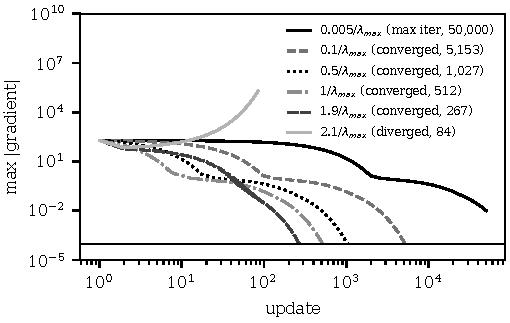
\includegraphics[width=\linewidth]{figures/fig_phase1.pdf}
    \caption{Phase 1 learning-rate comparison: $\max|\nabla J|$ per update (log--log); horizontal line: tolerance $10^{-4}$.}
    \label{fig:p1}
  \end{minipage}\hfill
  \begin{minipage}[t]{0.485\textwidth}
    \centering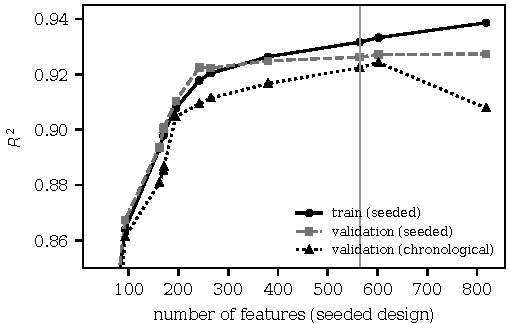
\includegraphics[width=\linewidth]{figures/fig_phase3.pdf}
    \caption{Phase 3 complexity sweep on both splits; vertical line: the \val{pThreeTargetN}-feature target.}
    \label{fig:p3}
  \end{minipage}
\end{figure}

\subsection{Phase 2: polynomial regression}
\textbf{Method.} Interaction groups were selected from Phase~1's training residuals: candidate groupings were ranked by the share of residual variance lying between group means (\val{stepAshare} for hour \x{} working day), adjusted for the number of groups and checked for sparse groups, and re-ranked after removing the confirmed groups. Degree was interpreted as interaction order, since powers of 0/1 indicators are uninformative. Products were formed from explicit term lists, never multiplying two levels of the same column. Every non-hour factor was centred at its training mean before multiplication, which leaves the representable predictions unchanged and lowered the condition number of the full design from \val{pTwoCondUnc} to \val{pTwoCond}. Each group was added in turn, every fit warm-started from the Phase~1 weights with new weights at zero (identical starting predictions were asserted) and run with the same $1.9/\lambda_{max}$ rule.

\textbf{Results.} Table~\ref{tab:p2} lists every step. Hour \x{} working day alone raised validation $R^2$ by \val{pTwoHrWdGain}. Degree~3 reached \val{pTwoDegThreeR} (RMSE \val{pTwoDegThreeRmse}, \val{pTwoDegThreeN} features, \val{pTwoDegThreeIter} updates). Its train--validation $R^2$ gap of \val{pTwoDegThreeGap} reflects sampling variation, as training and validation RMSE are nearly equal (\val{pTwoDegThreeTrainRmse} and \val{pTwoDegThreeValRmse}). The shortfall in the top predicted decile fell from \val{pTwoTopPredStart} to \val{pTwoTopPredEnd} bikes. \textbf{Passed on:} degree~3 and the \val{pTwoDegThreeN}-feature list with lineage, weights and scaler.

\begin{table}[t]
  \centering\small
  \caption{Phase 2: groups added in turn (validation unless marked).}
  \label{tab:p2}
  \begin{tabular}{@{}lrrrrr@{}}
    \toprule
    Model & Degree & Features & Train $R^2$ & Val.\ $R^2$ & Top-predicted-decile shortfall \\
    \midrule
    % Generated by report/build_report.py. Do not edit.
Phase 1 (main effects) & 1 & 47 & 0.6970 & 0.6823 & 134.9 \\
+ hour $\times$ workingday & 2 & 70 & 0.8316 & 0.8310 & 88.0 \\
+ hour $\times$ yr & 2 & 93 & 0.8641 & 0.8675 & 77.4 \\
+ hour $\times$ season & 2 & 162 & 0.8933 & 0.8937 & 56.5 \\
+ hour-block $\times$ weathersit & 2 & 170 & 0.8979 & 0.9004 & 54.1 \\
+ temp $\times$ hum & 2 & 171 & 0.8993 & 0.9009 & 53.8 \\
+ hour $\times$ workingday $\times$ yr & 3 & 195 & 0.9078 & 0.9105 & 50.4 \\
+ hour $\times$ workingday $\times$ temp & 3 & 242 & 0.9178 & 0.9225 & 43.3 \\
\bottomrule

  \end{tabular}
\end{table}

\subsection{Phase 3: bias--variance trade-off}
\textbf{Method.} The complexity sweep followed Phase~2's order and continued beyond it (hour \x{} holiday, hour \x{} weekday, hour \x{} month, full hour \x{} weather, and the degree-4 group hour \x{} working day \x{} year \x{} season) in order to reach the high-variance regime. Columns that were exact linear combinations of earlier ones were detected by QR factorisation and removed. Learning curves were computed for the degree-3 design and the largest design. The single chronological split held out the last 20\% of labelled days (\val{pThreeChronoDays} days, \val{pThreeChronoRows} hours, from \val{pThreeFirstDay}) as whole days, with all preprocessing refitted on the earlier days. The target rule was fixed before the run: the converged fit with the fewest features whose seeded validation $R^2$ lies within \val{rTol} of the best.

\textbf{Results.} Seeded validation $R^2$ rose from \val{pTwoDegThreeR} to a plateau of \val{pThreeDegFourR} at \val{pThreeDegFourN} features, while the train--validation gap widened to \val{pThreeDegFourGap} (Figure~\ref{fig:p3}); all fits converged (at most \val{pThreeMaxIter} updates). The degree-3 learning curve was flat with training and validation RMSE nearly equal, indicating a bias-limited model. The largest design showed a gap of \val{pThreeLcGapSmall} bikes at 25\% of the data that closed to \val{pThreeLcGapFull}, indicating a variance-limited model. On the chronological split degree~3 scored $R^2$ \val{pThreeDegThreeChronoR} (RMSE \val{pThreeDegThreeChronoRmse}), because it extrapolates into later and busier days. The extensions up to full hour \x{} weather improved the chronological score by \val{pThreeChronoGain} (seeded: \val{pThreeSeededGain}), whereas the degree-4 group reduced it by \val{pThreeDegFourChronoDrop} and increased the top-decile shortfall by \val{pThreeDegFourChronoShort} bikes: the earlier days contain no 2012 autumn hours, so these terms cannot be learned (\val{pThreeDegFourChronoN} instead of \val{pThreeDegFourN} features remain). Combinations observed in training therefore transferred; unobserved ones did not. \textbf{Diagnosis:} degree~3 is bias-limited and variance appears only at degree~4. \textbf{Passed on:} the \val{pThreeTargetN}-feature design ending at hour \x{} month (seeded $R^2$ \val{pThreeTargetR}, chronological \val{pThreeTargetChronoR}) and the noise candidate temp \x{} hum.

\subsection{Phase 4: regularisation}
\textbf{Method.} All methods minimised $J(w)=\lVert Xw-y\rVert^2/(2n)+\lambda\big[\rho\sum_{j\ge1}|w_j|+(1-\rho)\sum_{j\ge1}w_j^2/2\big]$ with an unpenalised intercept: Ridge ($\rho=0$), Lasso ($\rho=1$) and Elastic Net ($\rho\in\{0.1,0.5,0.9\}$). Each update takes a gradient step on the smooth part, in which the Ridge term adds $\lambda(1-\rho)$ to the diagonal of $H$, and then soft-thresholds: every penalised weight is moved towards zero by $\eta\lambda\rho$ and set to exactly zero if it would cross it. Ridge used $\eta=1.9/L$ and the L1-type methods $\eta=1/L$, with $L=\lambda_{max}+\lambda(1-\rho)$, so that the objective cannot increase. Each method followed a log-spaced $\lambda$ path from its largest value downwards (for Lasso, from $\lambda_{max}=\val{lassoLamMax}$, where all weights vanish), every fit warm-started from the previous one. The brief fixes a single validation set, so no $k$-fold cross-validation was used. Ridge was selected by the highest validation $R^2$; Lasso and Elastic Net by the largest $\lambda$ within \val{selTol} of the path's best $R^2$.

\textbf{Results.} In the first run all L1-type paths peaked at their last grid value; the paths were extended to $\lambda=10^{-5}$ at the same spacing, the first 30 values reproduced exactly, and only the Elastic Net choice changed. Table~\ref{tab:p4} and Figure~\ref{fig:p4} summarise the result. Ridge was best (validation $R^2$ \val{ridgeR} against \val{unpenR} unpenalised), Lasso retained \val{lassoN} of \val{pThreeTargetN} weights at \val{lassoR}, and Elastic Net selected $\rho=\val{enetRho}$. Phase~3 had left almost no variance to remove, so the penalty could only add bias: the top-decile shortfall rose from \val{unpenShort} to \val{lassoShort} bikes under Lasso. Column verdicts (Table~\ref{tab:verdicts}) combine a grouped ablation, in which the design is rebuilt without the column and every term derived from it and refitted with the Ridge setting, or an add-back test; the $R^2$ of the column alone in its full encoding; and Lasso survival. A column is \emph{useful} if its removal costs at least \val{rTol} in $R^2$, otherwise \emph{redundant} if its own $R^2$ is at least \val{aloneTol}, and otherwise \emph{uninformative}. \emph{holiday} retains most of its terms under Lasso yet costs nothing when removed: a surviving coefficient does not establish usefulness. \textbf{Passed on:} the \val{survivors} Lasso survivors (from \val{survivorColumns} original columns) with lineage; Ridge as the recommended regression model.

\begin{figure}[t]
  \centering
  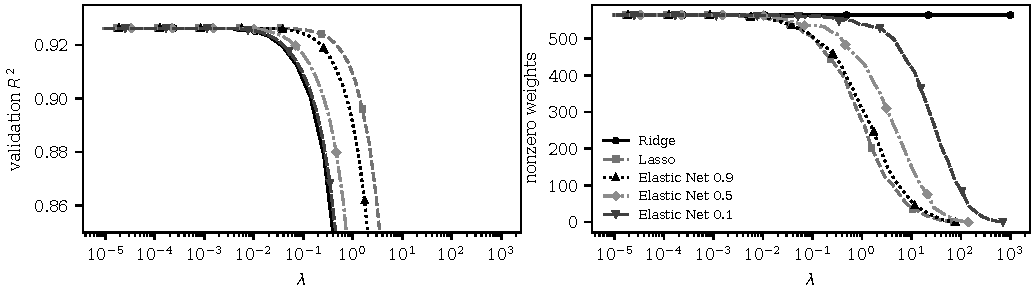
\includegraphics[width=\textwidth]{figures/fig_phase4.pdf}
  \caption{Phase 4 regularisation paths: validation $R^2$ and number of nonzero weights against $\lambda$.}
  \label{fig:p4}
\end{figure}

\begin{table}[t]
  \centering\small
  \caption{Phase 4: selected models (validation; shortfall: mean bikes missing in top-decile hours).}
  \label{tab:p4}
  \begin{tabular}{@{}lrrrrrr@{}}
    \toprule
    Method & $\lambda$ & $\rho$ & Nonzero weights & Val.\ $R^2$ & RMSE & Top-decile shortfall \\
    \midrule
    % Generated by report/build_report.py. Do not edit.
Unpenalised (Phase 3) & 0 & -- & 564 & 0.9262 & 49.9 & 53.8 \\
Ridge & 0.000452 & 0 & 564 & 0.9262 & 49.9 & 54.0 \\
Lasso & 0.169 & 1 & 466 & 0.9248 & 50.4 & 56.9 \\
Elastic Net & 0.0144 & 0.1 & 564 & 0.9246 & 50.5 & 57.6 \\
\bottomrule

  \end{tabular}

  \vspace{6pt}
  \caption{Column verdicts ($\Delta R^2$: change in validation $R^2$ against the Ridge model; Lasso: surviving terms derived from the column).}
  \label{tab:verdicts}
  \begin{tabular}{@{}llrrrl@{}}
    \toprule
    Column & Test & $\Delta R^2$ & Alone $R^2$ & Lasso & Verdict \\
    \midrule
    % Generated by report/build_report.py. Do not edit.
\texttt{instant} & add back & 0.0003 & 0.094 & -- & redundant \\
\texttt{dteday} & add back & 0.0002 & 0.094 & -- & redundant \\
\texttt{season} & removal & 0.0000 & 0.053 & 56/69 & redundant \\
\texttt{yr} & removal & $-$0.1103 & 0.067 & 45/48 & useful \\
\texttt{mnth} & removal & $-$0.0055 & 0.070 & 149/195 & useful \\
\texttt{hr} & removal & $-$0.5684 & 0.491 & 443/537 & useful \\
\texttt{holiday} & removal & $-$0.0000 & $-$0.000 & 18/24 & uninformative \\
\texttt{weekday} & removal & $-$0.0052 & $-$0.001 & 100/121 & useful \\
\texttt{workingday} & removal & $-$0.0162 & 0.000 & 63/71 & useful \\
\texttt{weathersit} & removal & $-$0.0175 & 0.016 & 9/10 & useful \\
\texttt{temp} & removal & $-$0.0143 & 0.165 & 42/49 & useful \\
\texttt{atemp} & add back & 0.0003 & 0.162 & -- & redundant \\
\texttt{hum} & removal & $-$0.0006 & 0.097 & 2/2 & redundant \\
\texttt{windspeed} & removal & $-$0.0006 & 0.015 & 1/1 & redundant \\
\bottomrule

  \end{tabular}
\end{table}

\subsection{Phase 5: logistic regression}
\textbf{Method.} An hour was labelled high demand if its count exceeded the 75th percentile of training hours in the same hour \x{} working-day \x{} year group (\val{labelGroups} cutoffs from the training portion, applied unchanged to validation). A single global cutoff would label \val{labelGlobalNever} of the 24 hours as never high, so the classifier would mainly learn the clock; a cutoff without year would label \val{labelNoYearOld}\% of 2011 and \val{labelNoYearNew}\% of 2012 hours as high. With the chosen label the rates are \val{labelOld}\% and \val{labelNew}\%, and \val{pFivePos} training hours (\val{pFivePosRate}\%) are positive (\val{pFiveValPos}\% in validation). The inputs were exactly the \val{survivors} Lasso survivors with the fitted scaler. The log-loss $-\frac{1}{m}\sum[y\log p+(1-y)\log(1-p)]$ with $p=\sigma(Xw)$ was minimised by gradient descent using the explicit gradient $X^\top(p-y)/m$. Its curvature is at most $L=\lambda_{max}(X^\top X/m)/4=\val{pFiveCurv}$, since $p(1-p)\le 1/4$, so the step $1.9/L=\val{pFiveLr}$ is safe. The probability cutoff maximised validation F-measure over 0.05--0.95.

\textbf{Results.} The fit converged in \val{pFiveIter} updates. ROC-AUC was \val{pFiveAuc}; at the tuned cutoff \val{pFiveCut}, accuracy was \val{pFiveAcc} against \val{pFiveBase} for always predicting ``not high'', precision \val{pFivePrec}, recall \val{pFiveRec} and F-measure \val{pFiveFone} (Table~\ref{tab:p5}, Figure~\ref{fig:p5}). At 0.5, accuracy was higher (\val{pFiveHalfAcc}) but the F-measure lower (\val{pFiveHalfFone}): \val{pFiveMissed} more busy hours were missed in exchange for \val{pFiveSavedAlarms} fewer false alarms. With a quarter of the hours positive, accuracy therefore rewards missing busy hours. Temperature had the largest odds ratio (\x\val{pFiveTempOdds} per standard deviation), followed by month indicators. The label still carries seasonality: \val{pFiveJan}\% of January and \val{pFiveJun}\% of June training hours are positive. A calendar-only ranking (month \x{} weekday) reaches ROC-AUC \val{pFiveAucCal}, whereas the classifier reaches \val{pFiveAucMonth} within a single month (\val{pFiveAucSeasonLo}--\val{pFiveAucSeasonHi} within a season), which measures its skill beyond the calendar.

\begin{figure}[t]
  \centering
  \begin{minipage}[t]{0.42\textwidth}
    \centering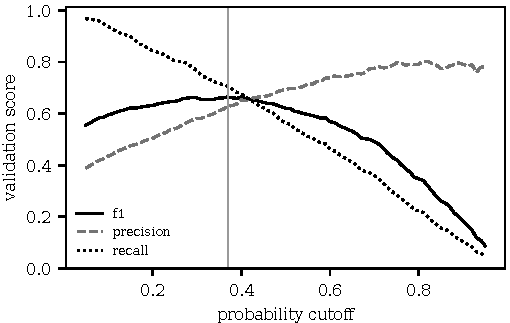
\includegraphics[width=\linewidth]{figures/fig_phase5.pdf}
    \caption{Phase 5 validation precision, recall and F-measure against the cutoff; vertical line: tuned cutoff.}
    \label{fig:p5}
  \end{minipage}\hfill
  \begin{minipage}[t]{0.55\textwidth}
    \centering\small
    \captionof{table}{Phase 5 confusion matrices and scores (validation).}
    \label{tab:p5}
    \begin{tabular}{@{}rrrrrrrrr@{}}
      \toprule
      Cutoff & TP & FP & FN & TN & Acc. & Prec. & Rec. & F1 \\
      \midrule
      % Generated by report/build_report.py. Do not edit.
0.37 & 388 & 230 & 161 & 1,399 & 0.820 & 0.628 & 0.707 & 0.665 \\
0.50 & 309 & 137 & 240 & 1,492 & 0.827 & 0.693 & 0.563 & 0.621 \\
\bottomrule

    \end{tabular}
  \end{minipage}
\end{figure}

\section{Bonus: asymmetric cost}
Under-prediction was assumed to cost three times as much as over-prediction of the same size, and the squared error was retained: $\ell(r)=\tfrac12 c(r)\,r^2$ with $r=\hat y-y$ and $c=3$ for $r<0$, otherwise $c=1$. The derivative $c(r)\,r$ is continuous, so the gradient is $X^\top(c\odot r)/n = X^\top r/n + 2X^\top\min(r,0)/n$, and its Lipschitz constant is $3\lambda_{max}$; the minimiser is the 0.75 expectile rather than the mean. A cost linear in the number of bikes would target the 75th percentile instead, but it has no gradient at zero, so fixed-step gradient descent could not converge on it. On Phase~1's features the Phase~1 learning rate diverged within \val{bDivIter} updates, whereas the rate divided by three (\val{bLr}) converged in \val{bIter} updates. Predictions rose by \val{bShift} bikes per hour on average. $R^2$ fell from \val{bRmse} to \val{bRasym} and RMSE rose from \val{bRmseMse} to \val{bRmseAsym}, as both measure the squared-error objective, while the asymmetric cost fell from \val{bCostMse} to \val{bCostAsym} (\val{bCostDrop}\%). Bikes short per hour fell from \val{bShortMse} to \val{bShortAsym}, idle bikes rose from \val{bIdleMse} to \val{bIdleAsym}, and the top-decile shortfall fell from \val{bTopMse} to \val{bTopAsym}. Because Phase~1 underfits, much of the lift went to hours that were already over-predicted. On Phase~2's features the same loss shifted predictions by only \val{fShift} bikes, cost \val{fRcost} in $R^2$ (from \val{fR}) and reduced the top-decile shortfall from \val{fTop} to \val{fTopAsym} bikes.

\section{Limitations}
\textbf{Seasonal label leakage.} The Phase~5 label removes the level of each hour, day type and year but not the season; a large part of the classifier's ROC-AUC (\val{pFiveAuc}) is reproducible from the calendar alone (\val{pFiveAucCal}). Adding season to the grouping would have produced many groups with too few rows for a stable percentile.
\textbf{Growth extrapolation.} On the chronological split the models under-predict their own busiest hours (mean error \val{pThreeTargetChronoErr} bikes in the top predicted decile for the target design, against \val{pThreeTargetSeededErr} on the seeded split), since growth beyond the training period cannot be extrapolated.
\textbf{One validation set.} $\lambda$, the Phase~3 target and the Phase~5 cutoff were tuned and scored on the same seeded validation set, so those scores are slightly optimistic.
\textbf{Phase 4 grid revision.} The L1-type $\lambda$ paths were extended after the first official run because their optima lay at the grid edge; the revision is recorded in the notebook and changed only the Elastic Net choice.

\section{Final submission}
The submitted predictions come from Phase~4's Ridge model ($\lambda=\val{ridgeLam}$) on the \val{pThreeTargetN}-feature design. With every choice frozen on the seeded split, the validation rows had served their purpose of selection, and the model was refitted on all \val{nAll} labelled hours by the same procedure, with encoders, scaler and centring means refitted on the combined rows (the same \val{sDropped} exact combinations were removed). The final fit converged in \val{sIter} updates (training $R^2$ \val{sR}, RMSE \val{sRmse}). The \val{nTest} test hours were predicted in the order of the sample file, and \val{sClipped} negative predictions were set to zero, since rentals cannot be negative (mean prediction \val{sMean}, maximum \val{sMax} bikes).

\end{document}
